\scanpage{138}
\margin{\uline{Remarque finale à 30} la formation des $\operatorname{tr}^*$ (et des ``traces \unsure{partielles}'') marche sur un espace annelé, avec hypothèse pseudo-cohérence \dots}
\margin{\textcircled{31}}
\uline{Complexes de Tor-dimension finie sur un préschéma}

$X$ préschéma, $L_\bullet\in\operatorname{Ob}D^-(X)$. On dit que \deleted{$X$}
$L_\bullet$ est de Tor dimension finie si pour tout
\deleted{faisceau}\inserted{Module} $F$ sur $X$, on a $\operatorname{Tor}_i(F,L_\bullet)=0$
pour \deleted{\unsure{$i$}}\inserted{$i$} grand. \inserted{(\unsure{compris aussi} \unsure{$-\infty$}, pour $|i|$ grand!)} De façon précise, on dit que
$L_\bullet$ est de \deleted{\unsure{Tor}} tor-dimension bornée par
$[N,\unsure{M|N'}]$, où \deleted{\unsure{$N\in\mathbb Z$}} $N,N'\in\mathbb Z$, si
\[
\operatorname{Tor}_i(F,L_\bullet)=0\quad\text{pour }i\notin[N,\unsure{M|N'}].
\]
\deleted{\unsure{Ceci posé,}}
On voit que ceci équivaut à dire
que pour tout pt géom $\bar x$ de $X$, le complexe
$L_{\bullet\bar x}$ est de tor-dim. bornée par
$[N,\unsure{M|N'}]$.
\deleted{\unsure{Cela} Cela signifie également, que}
\deleted{\unsure{si} $L_\bullet$ est plat (\unsure{ce qu'on peut en effet supposer}) \unsure{que}}
\deleted{\unsure{Pour} $L_\bullet$ est isomorphe à un complexe
$L'_\bullet$ tel que\quad a) $L'^i$}
\deleted{Dire que
la tor-dimension est\quad Si \unsure{$L_\bullet$}, est
plat (ce qu'on peut toujours supposer) alors
$L_\bullet$ est de tor-dim majorée par $[\deleted{\unsure{N}}-\infty,N']$
b) Si $L_\bullet$ est plat, alors dire que la}
\figure{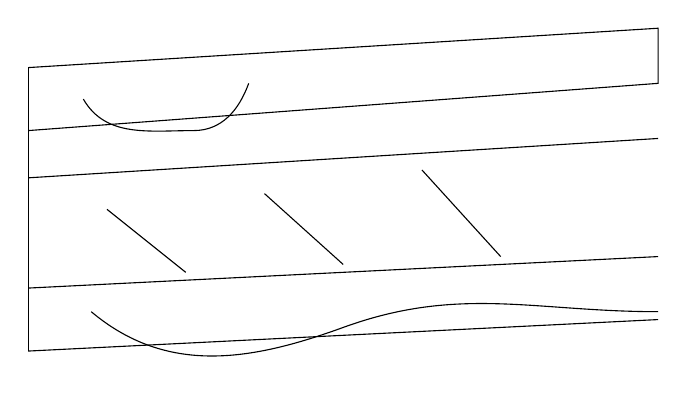
\begin{tikzpicture}\draw (0,0)--(0,-3.6);\draw (0,0)--(8,.5)--(8,-.2)--(0,-.8);\draw (0,-1.4)--(8,-.9);\draw (0,-2.8)--(8,-2.4);\draw (0,-3.6)--(8,-3.2);\draw (.7,-.4) to[out=-60,in=180] (2.1,-.8) to[out=0,in=-110] (2.8,-.2);\draw (1,-1.8)--(2,-2.6);\draw (3,-1.6)--(4,-2.5);\draw (5,-1.3)--(6,-2.4);\draw (.8,-3.1) to[out=-40,in=200] (4,-3.3) to[out=20,in=180] (8,-3.1);\end{tikzpicture}}
Cela signifie aussi que si
$L'_\bullet\in\operatorname{Ob}D^b$ a sa cohomologie bornée par $\unsure{[N',M']|[N',N_1]}$,
alors $L_\bullet\overset{\mathbb L}{\otimes}L'_\bullet$ a sa cohomologie bornée par
\mspage{137}
